\section{Ejercicio 2}

A continuación mostramos 3 corridas del algoritmo \textit{First-come, First-served}, con  una simulación de 1, 2 y 3 cores respectivamente:

\begin{figure}[h]
	\centering                                                       
	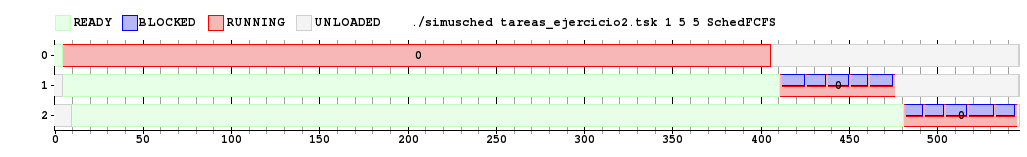
\includegraphics[width=450pt]{./figs/ejercicio2_1core.png}
\end{figure}

\begin{figure}[h]
	\centering                                                       
	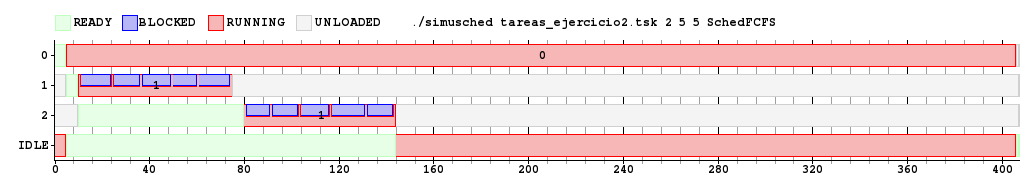
\includegraphics[width=450pt]{./figs/ejercicio2_2cores.png}
\end{figure}

\begin{figure}[h]
	\centering                                                       
	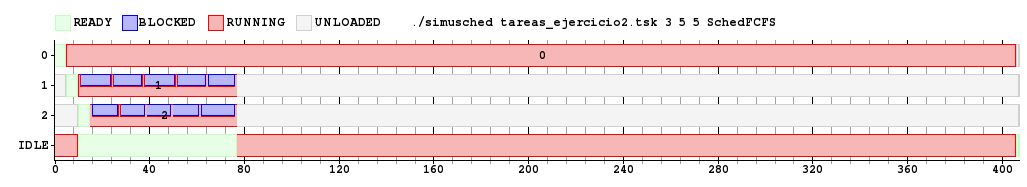
\includegraphics[width=450pt]{./figs/ejercicio2_3cores.png}
\end{figure}

Lo que se puede ver el primer gráfico es la corrida de las 3 tareas con un sólo núcleo. Estas tareas se corren de manera secuencial en el procesador y cuando termina una comienza la siguiente, siempre y cuando haya pasado el tiempo de inicio (sino es como si la misma no existiera). La primer tarea es la que usa constantemente el CPU durante un tiempo fijado (400) en el archivo del lote de tareas. Luego se ejecutan las tareas con interrupciones aleatorias (5 interrupciones con duraciones al azar entre 10 y 15ms).

En el segundo gráfico ya podemos ver cierto grado de multiprogramación, en el cual hay momentos con 2 tareas corriendo al mismo tiempo, en cada uno de los 2 cores que posee el sistema. El primer core se ocupa durante todo el tiempo de ejecución de la primera tarea, teniendo el segundo core, momentos donde ejecuta la segunda tarea, otros donde ejecuta la tercera y finalmente, tiempo idle en el que no hace nada.

En el tercer gráfico podemos ver nuevamente multiprogramación, pero esta vez con una mayor presencia de la tarea idle, ya que se corren al mismo tiempo las tareas de consola, terminando más rápido que en la simulación anterior. La tarea de CPU sigue tardando lo mismo que en los casos anteriores.

En todos los casos podemos ver el funcionamiento correcto del algoritmo FCFS, dado que las tareas se ejecutan en el mismo órden en el que llegan, como se esperaba.